Identification of the ball consists of two steps:
\begin{enumerate}
  \item Identifying the primary color of the ball
  \item Determining whether the ball is striped
\end{enumerate}
Both steps involves measuring the color distribution of the detected ball. The primary color in the distribution represents the color of the ball, while the amount of white in the distribution determines if the ball is striped.

\subsection{Vector Angle Versus Euclidean Distance}
The color of a ball has to be classified to one of the eight different ball colors. This is achieved by calculating distances between the detected ball and model colors obtained from ball calibration. The detected ball is then classified as the model that has the shortest distance.

There are different ways of measuring difference between colors, and each of these measurements has their own advantages. In this section two methods for measuring color difference are compared to find the one most suitable for ball classification.

If we define two color vectors as $v_{1}$ and $v_{2}$, the euclidean distance between them is defined as
\begin{equation}
D_{E}(v_{1}, v_{2}) = ||v_{1}, v_{2}||
\end{equation}
where $||\bullet||$ is the $L_{2}$ vector norm. For the RGB coordinate system where $v = [r\;g\;b]^{T}$, the distance is calculated as
\begin{equation}
D_{E}(v_{1}, v_{2}) = \sqrt{(r_{1} - r_{2})^{2} + (g_{1} - g_{2})^{2} + (b_{1} - b_{2})^{2}}
\end{equation}
In RGB space the euclidean distance is more sensitive to differences in intensity than differences in color. This can cause problems if a light version of a color should match a darker version. Another measure, that does a better job of quantifying chromaticity difference in RGB space is the vector angle which is calculated as
\begin{equation}
cos \theta = \frac{v_{1}^ Tv_{2}}{||v_{1}|| ||v_{2}||}
\end{equation}
The vector angle between two colors having the same chromaticity but different intensity will be the same, as seen in figure \ref{fig:angleVersusEuclideanDrawing}. The vector angle in RGB is equivalent to using the hue distance in HSB. Using the vector angle instead of converting the entire image to HSB can save computation time.\cite{angleVsEuclidean}
\begin{figure}[H]
  \centering
  \subfloat[Visual representation of color distance]{\label{fig:angleVersusEuclideanDrawing}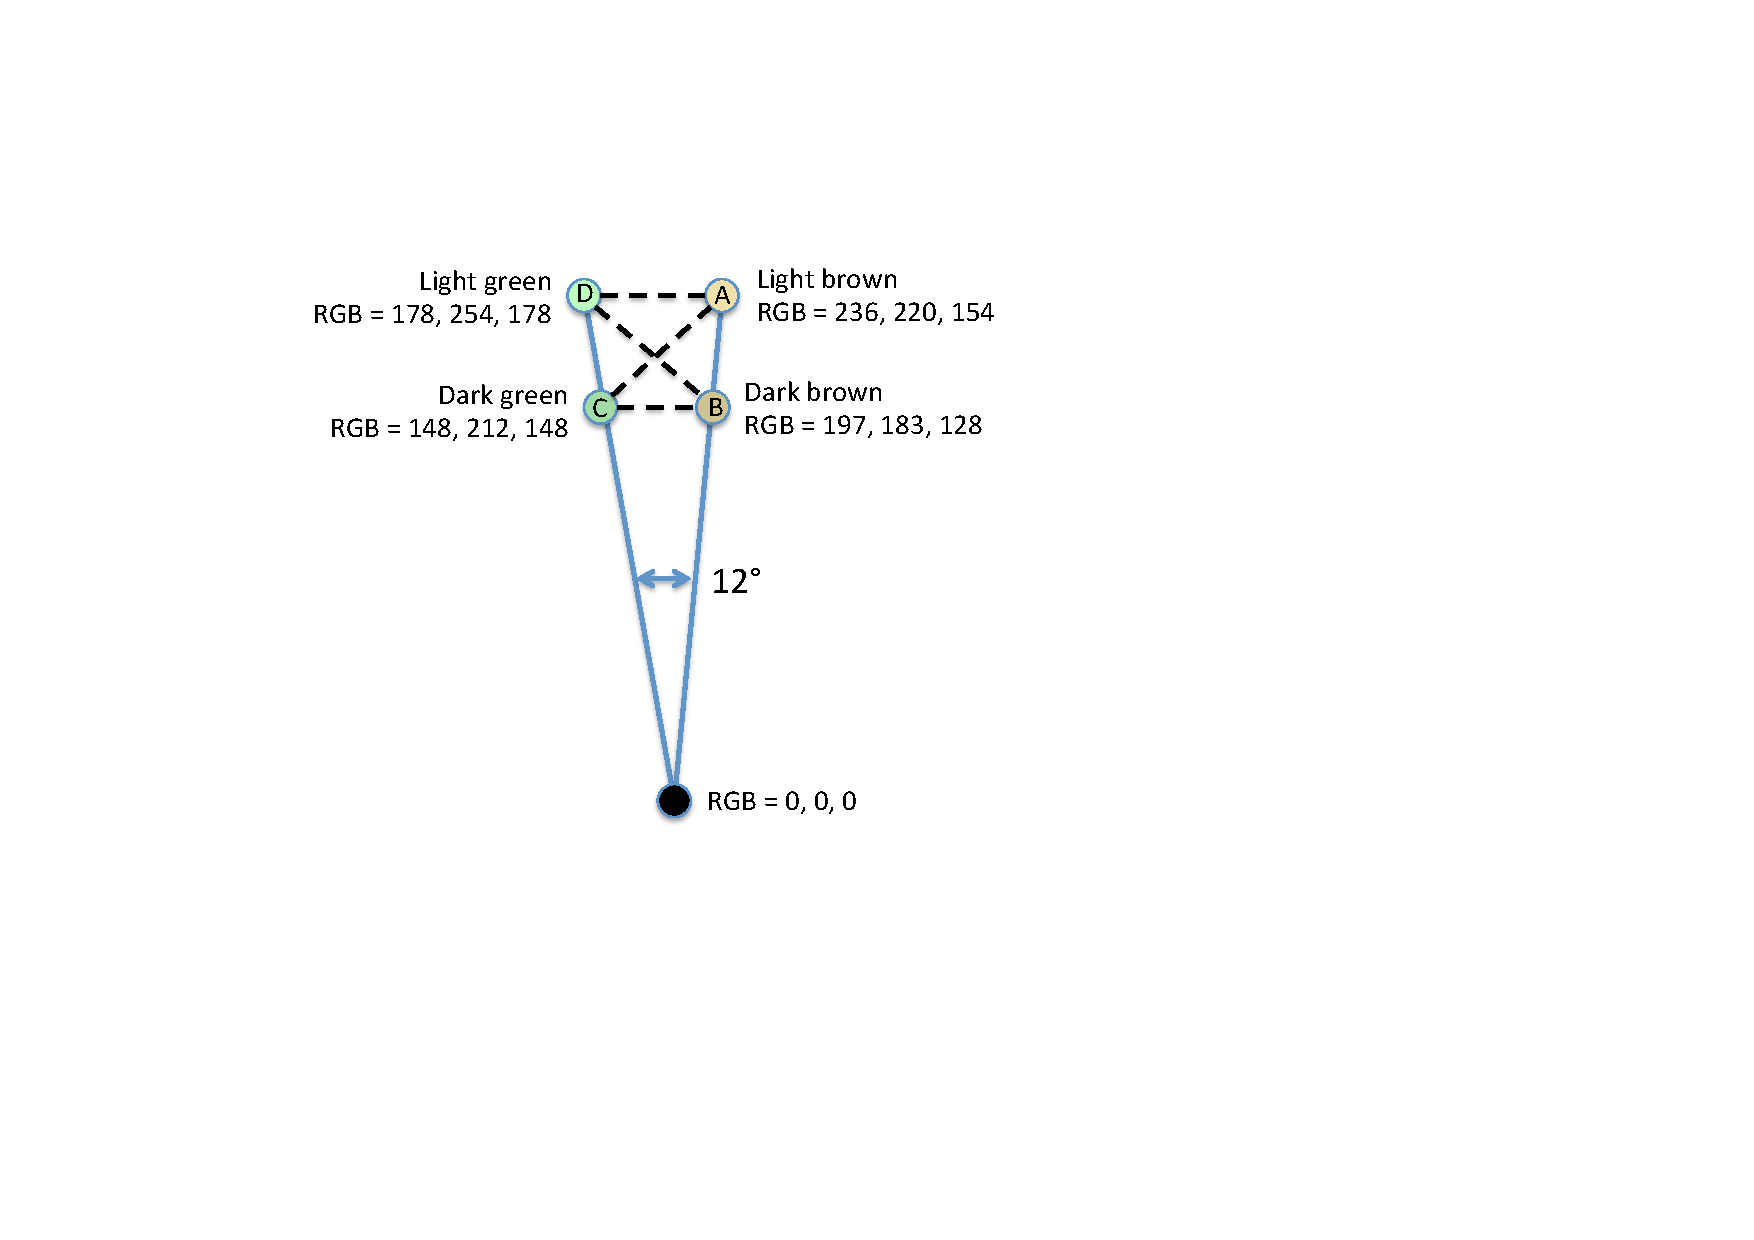
\includegraphics[width=0.38\textwidth]{images/angleVersusEuclidean}}
  \quad           
  \subfloat[Euclidean distances]{
  	\label{tab:angleVersusEuclidean}
	\begin{tabular}[b]{|c|c|c|c|c|}
		\hline
		- & A 		& B 	& C 	& D		\\
		\hline
		A & 0		& 59.7 	& 88.6 	& 71.4	\\
		\hline
		B & 59.7	& 0 	& 60.3 	& 88.9	\\
		\hline
		C & 88.6 	& 60.3 	& 0 	& 59.7	\\
		\hline
		D & 71.4 	& 88.9 	& 59.7 	& 0		\\
		\hline
	\end{tabular}
}
\caption{Example of differences between angular and euclidean distances.}
\label{fig:angleVersusEuclidean}
\end{figure}
As written in section \ref{sec:analballs} regarding ball analysis, the balls should be separable in hue-saturation space, and thereby also separable by vector angle comparison. Experiments with both distances did however conclude that the angular distance between balls having similar hue was to short to give a robust classification. The vector angle, was for this reason abandoned, and the euclidean distance was used in the final implementation.

\subsection{Color Comparison Strategy}

The ball color can be measured in two different ways: 
\begin{enumerate}
  \item Measure the distribution of the detected ball
  \item Use each pixel in the ball by itself
\end{enumerate}

The difference between the distribution of the detected ball and the model distributions can be measured using, e.g. Bhattacharyya or earth mover's distance. In this project, simpler metrics like the mean and the max has been used to compare ball distributions. 

Another way of looking at a ball is pixel by pixel. Each pixel is classified by itself, and the ball class is selected by taking the class where most of the ball pixels belong to. This is the approach used in this project. The thought behind this approach is that it will perform better against outliers and the varying number of colored pixels that is the nature of the pool balls. 

\subsection{Implementation}
The classifier is trained by supervised training where the user selects the location for each of the solid colored balls. The mean RGB value is then extracted from each of the ball areas and this will serve as a model for color comparison. \fxnote{Figure showing sampling of color means from image during calibration}
The euclidean distance between al each pixel and the models are calculated to determine the ball that the pixel is most likely to represent.

\begin{table}[htpb]
\begin{center}
	\begin{tabular}{|l|c|c|c|c|c|c|c|c|c|}
		\hline
		Ball & c & \cellcolor{yellow}1 & \cellcolor{blue}2 & \cellcolor{red}3  & \cellcolor{purple}4 & \cellcolor{orange}5 & \cellcolor{green}6 & \cellcolor{brown}7 & \cellcolor{black}\textcolor{white}{8} \\
		\hline
		
\includegraphics[]{images/ballsInVotes/0} & \cellcolor{gray}450 & 0 & 2 & 0 & 0 & 8 & 77 & 3 & 36\\
		\hline
		
\includegraphics[]{images/ballsInVotes/1} & 5 & \cellcolor{gray}420 & 1 & 0 & 1 & 15 & 64 & 35 & 35\\
		\hline
		
\includegraphics[]{images/ballsInVotes/2} & 15 & 0 & \cellcolor{gray}437 & 0 & 37 & 6 & 32 & 0 & 49\\
		\hline
		
\includegraphics[]{images/ballsInVotes/3} & 11 & 0 & 20 & \cellcolor{gray}333 & 34 & 51 & 12 & 113 & 2\\
		\hline
		
\includegraphics[]{images/ballsInVotes/4} & 19 & 0 & 87 & 0 & \cellcolor{gray}293 & 8 & 24 & 3 & 142\\
		\hline
		
\includegraphics[]{images/ballsInVotes/5} & 2 & 0 & 16 & 27 & 12 & \cellcolor{gray}452 & 23 & 34 & 10\\
		\hline
		
\includegraphics[]{images/ballsInVotes/6} & 35 & 0 & 9 & 0 & 0 & 3 & \cellcolor{gray}504 & 1 & 24\\
		\hline
		
\includegraphics[]{images/ballsInVotes/7} & 0 & 0 & 18 & 13 & 54 & 18 & 14 & \cellcolor{gray}413 & 46\\
		\hline
		
\includegraphics[]{images/ballsInVotes/8} & 21 & 0 & 27 & 0 & 33 & 12 & 74 & 12 & \cellcolor{gray}397\\
		\hline
		
\includegraphics[]{images/ballsInVotes/9} & \cellcolor{gray}170 & \cellcolor{gray}291 & 0 & 0 & 0 & 3 & 74 & 18 & 20\\
		\hline
		
\includegraphics[]{images/ballsInVotes/10} & \cellcolor{gray}145 & 1 & \cellcolor{gray}232 & 0 & 40 & 16 & 66 & 9 & 67\\
		\hline
		
\includegraphics[]{images/ballsInVotes/11} & \cellcolor{gray}94 & 3 & 5 & \cellcolor{gray}229 & 7 & 109 & 30 & 65 & 34\\
		\hline
		
\includegraphics[]{images/ballsInVotes/12} & \cellcolor{gray}142 & 0 & 6 & 0 & 106 & 21 & 82 & 25 & \cellcolor{red}194\\
		\hline
		
\includegraphics[]{images/ballsInVotes/13} & \cellcolor{gray}256 & 2 & 7 & 2 & 23 & \cellcolor{gray}177 & 37 & 54 & 18 \\
		\hline
		
\includegraphics[]{images/ballsInVotes/14} & \cellcolor{gray}253 & 0 & 9 & 0 & 1 & 6 & \cellcolor{gray}202 & 3 & 102\\
		\hline
		
\includegraphics[]{images/ballsInVotes/15} & \cellcolor{gray}107 & 0 & 7 & 14 & 19 & 47 & 49 & \cellcolor{gray}311 & 22\\
		\hline
	\end{tabular}
\end{center}
	\label{table:ballvote}
	\caption{Detected balls and their votes. Gray shading marks a correct identification.}
\end{table}
Table \ref{table:ballvote} shows the votes for the detected balls in a session where all 16 balls were present on the table. Each of the balls are identified by the maximum number of votes for a color, indicated by a gray background for a correct match, and red for incorrect match. Balls having white votes above a certain threshold are classified as striped balls, indicated by a gray background in both their primary color and cue.

In the situation seen in table \ref{table:ballvote} the only error comes from the striped purple 14 being identified as the black. The same problem is spotted in the solid variant: the purple 6, which also has a high number of black votes. The solid balls has more colored pixels to represent the color, making the problem worst among striped balls.
\fixme{table ref}